\documentclass[12pt]{article}

% packages

%\usepackage{times} % alt: cmbright
\usepackage[top=1in, bottom=1in, left=1in, right=1in]{geometry}
\usepackage{natbib}
\usepackage{amsmath}
\usepackage{amssymb}
\usepackage{latexsym}
\usepackage{sectsty}
\usepackage{amsfonts}
\usepackage{epsfig}
\usepackage{url}
\usepackage{microtype}
\usepackage{fixmath}
\usepackage{hyperref}
\usepackage{amsthm}
\usepackage{subfigure}
\usepackage{float}
\usepackage{hyperref}

\newtheorem{lem}{Lemma}
\newtheorem{defn}{Assumption}
\newtheorem{propty}{Property}
\newtheorem{thm}{Theorem}

% references

\newcommand{\mysec}[1]{Section~\ref{sec:#1}}
\newcommand{\myapp}[1]{Appendix~\ref{app:#1}}
\newcommand{\myeq}[1]{Equation~\ref{eq:#1}}
\newcommand{\myeqp}[1]{Eq.~\ref{eq:#1}}
\newcommand{\mychap}[1]{Chapter~\ref{chap:#1}}
\newcommand{\myfig}[1]{Figure~\ref{fig:#1}}

% math conveniences

\newcommand{\g}{\,\vert\,}
\newcommand{\E}{\textrm{E}}
\newcommand{\vct}[1]{\textbf{#1}}
\newcommand{\realline}{\mathbb{R}}
\newcommand{\indpt}{\protect\mathpalette{\protect\independenT}{\perp}}
\def\independenT#1#2{\mathrel{\rlap{$#1#2$}\mkern2mu{#1#2}}}
\newcommand{\h}[1]{\textrm{H}\left( #1 \right)}
\newcommand{\half}{\frac{1}{2}}
\newcommand{\new}{\textrm{new}}

\newcommand{\mult}{\textrm{Mult}}
\newcommand{\dir}{\textrm{Dir}}
\newcommand{\discrete}{\textrm{Discrete}}
\newcommand{\Bern}{\textrm{Bern}}
\newcommand{\DP}{\textrm{DP}}
\newcommand{\GP}{\textrm{GP}}
\newcommand{\Bet}{\textrm{Beta}}

% paragraph spacing

\setlength{\parindent}{0pt}
\setlength{\parskip}{2ex plus 0.5ex minus 0.2ex}

\allsectionsfont{\sffamily\mdseries}
\paragraphfont{\sffamily\bfseries}

\usepackage{algorithm}
\usepackage{algorithmic}
\renewcommand{\algorithmicrequire}{\textbf{Input:}}
\renewcommand{\algorithmicensure}{\textbf{Output:}}


\begin{document}

\title{\textsf{Convergence of Particle Swarms to Pareto Front in Multi-Objective Optimization}}
\author{\textsf{Daqing Yi}}
\date{\textsf{CS611 Assignment 2 - Rough Draft}}

\maketitle

%\section{Requirement}
%\begin{itemize}
%\item Write a concise, formal and accurate statement of your theorem 
%\item Include with this a set of brief definitions (formal, if possible, informal when necessary for brevity) that will allow a reader to understand the content and significance of your statement
%\end{itemize}


\section{Definitions}

\begin{prop}[\textbf{Minimum Problem}]
All the optimization functions in this paper are defined for minimum problems.
\end{prop}
A solver of a minimum problem can be converted to a solver of a maximum problem easily.

\begin{mydef}[\textbf{Multi-Objective Optimization}]
\label{def:multi_opt}
Find the vector $ \vec{x}^{*} = \left[ {x}_{1}^{*}, {x}_{2}^{*}, \cdots {x}_{n}^{*} \right]^{T} \in \Omega $, which will satisfy the $ m $ inequality constraints
\begin{equation}
\label{eq:mo_ineq_constraint}
g_{i}(\vec{x}) \geq 0, i = 1, 2, \cdots , m, 
\end{equation}
the $ p $ equality constraints
\begin{equation}
\label{eq:mo_eq_constraint}
h_{i}(\vec{x}) = 0, i = 1, 2, \cdots , p, 
\end{equation}
and will optimize the vector function
\begin{equation}
\label{eq:mo_obj}
\min_{\Omega} \vec{f}(\vec{x}) = \left[ f_{1}(\vec{x}), f_{2}(\vec{x}) \cdots f_{k}(\vec{x}) \right]^{T},
\end{equation}
where $ \vec{x} = \left[ x_{1}, x_{2}, \cdots x_{n} \right]^{T} $ is the vector of decision variables.
\end{mydef}

\begin{mydef}[\textbf{Pareto dominance}]
\label{def:pareto_dom}
A vector $ \vec{x} $ dominates a vector $ \vec{x}' $, denoted by $ \vec{x} \prec \vec{x}' $, if and only if 
\begin{itemize}
\item $ \vec{x} $ is not worse than $ \vec{x}' $ in all objectives, i.e. $ \forall i = 1, \cdots, k, f_{i}(\vec{x}) \leq f_{i}(\vec{x}') $, 
\item $ \vec{x} $ is strictly better than $ \vec{x}' $ in at least one objective, i.e. $ \exists i = 1, \cdots , k, f_{i}(\vec{x}) < f_{i}(\vec{x}') $. 
\end{itemize}
\end{mydef}

\begin{prop}[\textbf{Strict dominance}]
In this paper, only strict dominance ($ \prec $) is considered for simplification. However, weak dominance ($ \preceq $) can be easily generalized from any conclusion reached.
\end{prop}

\begin{mydef}[\textbf{Pareto optimal}]
\label{def:pareto_opt}
$ \vec{x}^{*} \in \Omega $ is \emph{Pareto optimal} if there does not exist a vector that dominates it, which is $ \nexists \vec{x}', \vec{x}' \preceq \vec{x}^{*} $.
\end{mydef}


\begin{mydef}[\textbf{Pareto optimal set}]
\label{def:pareto_opt_set}
For a given Multi-Objective Optimization problem $ \vec{f}(\vec{x}) $, the \emph{Pareto optimal set} $ P^{*} $ is defined as
\begin{equation}
\label{eq:pa_opt_set}
P^{*} := \{ \vec{x} \in \Omega \mid \neg \exists \vec{x}' \in \Omega (\vec{x}' \preceq \vec{x}) \}.
\end{equation}

\end{mydef}

\begin{mydef}[\textbf{Pareto Front}]
\label{def:pareto_front}
For a given Multi-Objective Optimization problem $ \vec{f}(\vec{x}) $ and Pareto optimal set $ P^{*} $, the \emph{Pareto front} $ PF^{*} $ is defined as
\begin{equation}
\label{eq:pa_front}
PF^{*} := \{ \vec{u} = \vec{f}(\vec{x}) \mid \vec{x} \in P^{*}  \}.
\end{equation}
\end{mydef}

\begin{mydef}[\textbf{Particle Swarm Optimization}]
\label{def:pso}
A \emph{particle} is a data structure that maintains current position $ \hat{\vec{x}} $ and current velocity  $ \hat{\vec{v}} $. Denote $ p_{best} $ for ``personal best'', which is the most fit position remembered by a particle. Denote $ g_{best} $ for ``global best'', which is most fit $ p_{best} $ among all particles. 
\begin{enumerate}
\item Scatter particles in decision space stochastically;
\item Each particle updates its location over time \\

\begin{subequations}
\label{eq:pso_alg}
\begin{align}
\vec{v}_{t+1} & = \omega \vec{v}_{t} + \phi_{1} U_{1}() (p_{best} - \vec{x}_{t}) + \phi_{2} U_{2}() (g_{best} - \vec{x}_{t}), \label{eq:pso_alg-1} \\
\vec{x}_{t+1} & = \vec{x}_{t} + \vec{v}_{t+1}  \label{eq:pso_alg-2},
\end{align}
\end{subequations}

in which $ U() $ is sampling from uniform distribution $ [0, 1] $.
\end{enumerate}
\end{mydef}

\section{Convergence problem in multi-objective optimization}

Convergence in particle swarm optimization means the swarm progresses towards a stable state. Analyzing the convergence problem of a given particle swarm optimization can be slitted into two phases, which answer separately:
\begin{enumerate}
\item whether the particle swarm converges;
\item and where the particle swarm converges to.
\end{enumerate}

The convergence of the particle swarm guarantees the usability of an algorithm on a problem. Where the particle swarm converges to determines the performance of an algorithm. In a single-objective optimization problem, the stable state that the swarm converges to can be a local optimum, a global optimum or weighted average between the local optimum and the global optimum.

Different from a single-objective optimization problem, the main objective of an algorithm for a multi-objective optimization problem is to find a set of non-dominated solutions to approximate the Pareto front. We expect the swarm to converge to a non-dominated solution set, which approximates the pareto front. The criteria for the non-dominated solution set can be defined as 
\begin{itemize}
\item minizing the average distance between solution set and the Pareto front; 
\item maximizing the diversity of the solution set;
\item and maintaining already found non-dominated solutions.
\end{itemize}

In this paper, I focus on analyzing the performance on minimizing average distance between solution set and the Pareto front, which can be represented as the centroid of the swarm converge to the centroid of the Pareto front. Considering the particles in a swarm as samples from distribution, the aim to prove is the convergence of the mean of the estimated distribution represented by particle sampling. In order to maximize the diversity, it is expected that the variance of the estimated distribution represented by particle sampling, which will not be explored here.

\section{Related work}

Compared with versatile algorithm modifications and applications in various fields, the works on dynamics and convergence analysis of particle swarm optimization are limited, and mostly are based on standard PSO. As defined in Equation \eqref{eq:pso_alg-1} and \eqref{eq:pso_alg-2}, the stochastic factor and non-linear terms imported by ``global best'' and ``personal best'' make it hard to apply common dynamics analysis methods.

% works on convergence in single-objective 
Focusing on search stagnation, which means no better solution is found, \cite{clerc2002particle} model ``global best'' and ``personal best'' as constants to convert this problem into time-invariant linear system analysis. Based on the same assumption, \cite{trelea2003particle} looks at dynamic behaviors of systems with different parameters. Considering a particle swarm as sampling from a problem space, \cite{poli2008dynamics} imports first and second order moments of the sampling distribution, which models the dynamics for convergence analysis. \cite{jiang2007stochastic} addresses the problem by looking at the convergence of variance. \cite{samal2007closed} considers the nonlinear terms ``global best'' and ``personal best'' as a control module, so the PSO system can be viewed as a closed-loop control system. Then the convergence problem is turned into stability problem in a closed-loop control system. 


% works on convergence in multi-objective
Analyzing dynamics in multi-objective optimization meets more complicate fitness function, which makes the ``global best'' and ``personal best'' vague. Because convergence target is no longer a single state but a solution set. A simple way is converting a multi-objective optimization problem to a weighted single objective optimization problem. 


\section{Maximin fitness function}

To solve a multi-objective optimization problem, a maximin fitness function is used in [\cite{li2004better}], which has the unique property of reward diversity and penalization of clustering of non-dominated solutions. In a population size of $ N $, the maximin fitness function is defined as:

\begin{equation}
\label{eq:maximin_fitness}
f_{maximin}(x) = \max_{j=1, \cdots, N} \{ \min_{i=1, \cdots , k}  ( f_{i}(x) - f_{i}(x_{j}) )  \}.
\end{equation}

Equation \eqref{eq:maximin_fitness} guarantees that the maximin fitness values of all non-dominated solutions are greater than zero.

Unlike the common way of defining a fitness function, the value of a fitness function is dependent with the distribution of other particles. Which means that the global best does not exist?

\subsection{Why Maximin}

TODO: explain why maximin works here

\begin{figure}
\centering
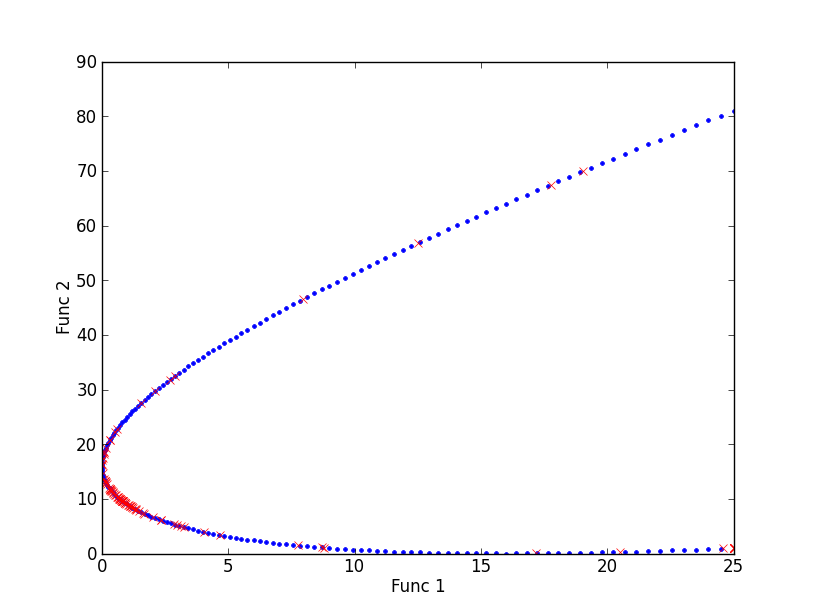
\includegraphics[width=0.7\linewidth]{./C1}
\caption{PSO-maximin on MOO}
\label{fig:C1}
\end{figure}



\section{Hypothesis}

Applying the maximin fitness function defined in Equation \eqref{eq:maximin_fitness} to particle swarm optimization defined in Equations \eqref{eq:pso_alg-1} and \eqref{eq:pso_alg-2}, the centroid of particles will converge to the centroid of Pareto front.

\section{Proof strategy}

\begin{enumerate}
\item Model the influence from ``global best'' and ``personal best'' in dynamic analysis. \\
$ g_{best} $ is denoted as some fixed but unknown parameter of the system. \\
$ p_{best} $ is denoted as a value determined by a monotonically increasing function through time. \\
Define $ \Delta\vec{x}_{t} = g_{best} - \vec{x}_{t} $, which shows how the current state approaches the ``global best''.
Then I can have
\begin{equation}
\label{eq:delta_gb}
g_{best} - \vec{x}_{t} = \Delta\vec{x}_{t},
\end{equation}
and  
\begin{equation}
\label{eq:delta_pb}
p_{best} - \vec{x}_{t} = p_{best} - g_{best} + \Delta\vec{x}_{t}.
\end{equation}

Apply Equation \eqref{eq:delta_gb} and \eqref{eq:delta_pb} to Equation \eqref{eq:pso_alg-2}, we have
\begin{equation}
\label{eq:trans_vel}
\begin{aligned}
\vec{v}_{t+1}  & = \omega \vec{v}_{t} + \phi_{1} U_{1}() (p_{best} - g_{best} + \Delta\vec{x}_{t}) + \phi_{2} U_{2}() (\Delta{\vec{x}_{t}}) \\
& = \omega \vec{v}_{t} + (\phi_{1} U_{1}() + \phi_{2} U_{2}()) \Delta\vec{x}_{t} + \phi_{1} U_{1}() (p_{best} - g_{best}).
\end{aligned}
\end{equation}

Apply Equation \eqref{eq:pso_alg-1} to Equation \eqref{eq:delta_gb}, we have
\begin{equation}
\label{eq:trans_del_pos}
\begin{aligned}
\Delta \vec{x}_{t+1} & = g_{best} - \vec{x}_{t+1} \\
& = g_{best} - \vec{x}_{t} - \vec{v}_{t+1} \\
& = \Delta \vec{x}_{t} - \vec{v}_{t+1}.
\end{aligned}
\end{equation}

Apply Equation \eqref{eq:trans_vel} to Equation \eqref{eq:trans_del_pos}, we have
\begin{equation}
\label{eq:trans_del_pos2}
\Delta \vec{x}_{t+1} = (1 - \phi_{1} U_{1}() - \phi_{2} U_{2}()) \Delta \vec{x}_{t} - \omega \vec{v}_{t} + \phi_{1} U_{1}() (g_{best} - p_{best}).
\end{equation}

Thus, we can have
\begin{equation}
\label{eq:linear_sys}
\begin{bmatrix}
\Delta \vec{x}_{t+1}
\\
\vec{v}_{t+1}
\end{bmatrix}
 = 
\begin{bmatrix}
1 - \phi_{1} U_{1}() - \phi_{2} U_{2}() &  - \omega
\\
\phi_{1} U_{1}() + \phi_{2} U_{2}() & \omega
\end{bmatrix}
*
\begin{bmatrix}
\Delta \vec{x}_{t}
\\
\vec{v}_{t}
\end{bmatrix}
+
\begin{bmatrix}
\phi_{1} U_{1}()
\\
- \phi_{1} U_{1}()
\end{bmatrix}
(g_{best} - p_{best})
\end{equation}


We can create a linear system expression using $ \Delta x_{t} $ instead of $ x_{t} $, which is expected to converge to zero, like the way of analyzing the error convergence in a linear control system.

At the same time, consider $ p_{best} - x_{t} $ as input to this linear control system, as shown in Fig. \ref{fig:system}. 

\begin{figure}
\centering
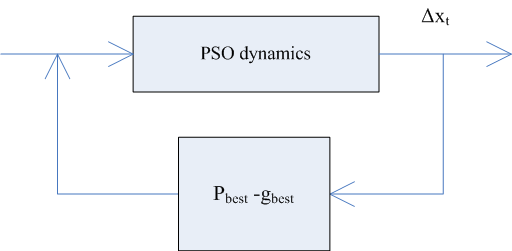
\includegraphics[width=0.7\linewidth]{./system}
\caption{Model the PSO dynamic as discrete linear system with feedback input}
\label{fig:system}
\end{figure}

\item Convert swarm dynamic to the mean of the particles' dynamics. \\

Model the $ U() $ in Equation \eqref{eq:pso_alg-2} as noise of input. As it is sampling between $ [0, 1] $, it can be converted into constant. Thus the stochastic factor in the linear expression can be eliminated.
 
\item Discrete system stability analysis. \\

Apply ``z-transform'' on this discrete linear system so that frequency-domain analysis can be applied for dynamics and convergence. 



\end{enumerate}



\bibliographystyle{apalike}
\bibliography{reference}

\end{document}
